%\RequirePackage[l2tabu, orthodox]{nag}
\documentclass[12pt,a4paper]{scrartcl}
\usepackage[colorlinks=true,
	linkcolor=black,
	citecolor=black,
	filecolor=black,
	urlcolor=blue,
	bookmarks=true,
	bookmarksopen=true,
	bookmarksopenlevel=3,
	plainpages=false,
	pdfpagelabels=true]{hyperref}
\usepackage[ngerman]{babel}				% Deutsche Sprachanpassungen
\usepackage[utf8]{inputenc}		% Direkte Angabe von Umlauten im Dokument. 
\usepackage[T1]{fontenc}
%\usepackage{lmodern}

\usepackage{lipsum}      % \lipsum
\usepackage{fancyvrb}    % \begin{Verbatim}
\usepackage{cprotect}    % verb in fbox

\usepackage{subcaption}  % subfigures

% Mathematische Symbole, Zeichen etc
\usepackage{amsmath}
\usepackage{amssymb}
\usepackage{amsthm}
\usepackage{bm}

\usepackage{pdfsync}
\usepackage{graphicx}

%\usepackage[activate={true,nocompatibility},final,tracking=true,kerning=true,spacing=true,factor=1100,stretch=10,shrink=10]{microtype}


\usepackage{todonotes}  % \todo{}

\title{Mein erstes Protokoll mit \LaTeX{}\\
Der sechsseitige Würfel}
\author{\begin{tabular}{l l} Praktikanten:& Hans Maulwurf\\
		Betreuer:& Homer Simpson
\end{tabular}}
\date{\today}

\begin{document}

%%%% Titelseite
\begin{titlepage}
    \maketitle
    \thispagestyle{empty}
\end{titlepage}
%%%% Titelseite

\setcounter{page}{1}    %    Seitenzahl wieder auf 1 setzen

\tableofcontents     %Inhaltsverzeichnis
\newpage
%%%%%%%%%%%%%%%%%%%%%%%%%%%%%%%%%%%%%%%%%%%%%%%%%%%%%%%%%%%%%%%%%%%%%%%%%%%
%Anfang des eigentlichen Dokumentes
%%%%%%%%%%%%%%%%%%%%%%%%%%%%%%%%%%%%%%%%%%%%%%%%%%%%%%%%%%%%%%%%%%%%%%%%%%%
\noindent Packages:
\begin{Verbatim}[frame=single]
\documentclass[12pt,a4paper]{scrartcl}
\usepackage[ngerman]{babel} % Deutsche Sprachanpassungen
\usepackage[utf8]{inputenc} % Direkte Angabe von Umlauten im Dokument. 
\usepackage[T1]{fontenc}

\usepackage{amsmath}  % Mathe
\usepackage{hyperref} % Links
\usepackage{graphicx} % z.B. .jpg Bilder einbinden
\end{Verbatim}
~\\
Zur Titelseite:\\~\\
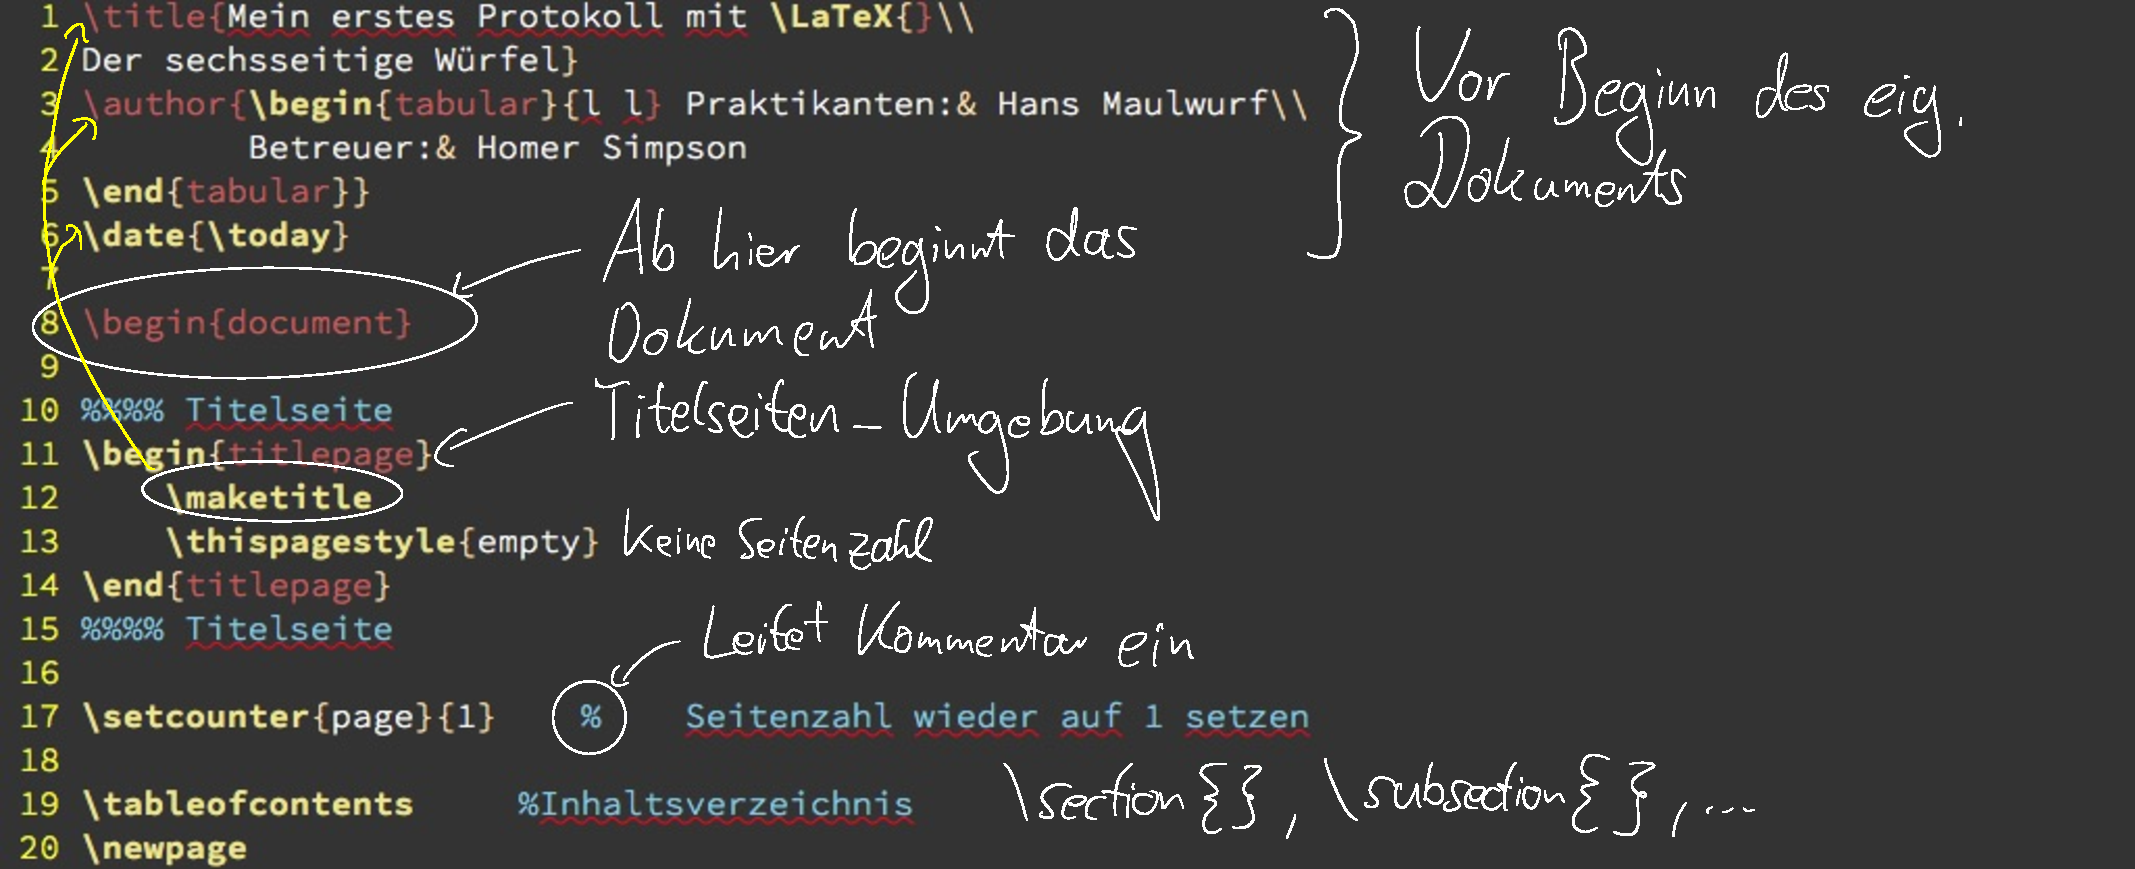
\includegraphics[width=1.1\textwidth]{figures/titelseite.pdf}
Natürlich kann man sich auch seine eigene Titelseite bauen, ohne
auf \verb!\maketitle! zurückzugreifen.

\section[Geschichte des Glücksspiels]{Geschichte des Glücksspiels \quad
$\leftarrow$ Section}
\subsection[Einführung]{Einführung \quad $\leftarrow$ Subsection}
\cprotect\fbox{
    \begin{minipage}{\textwidth}
        In diesem Abschnitt lernen wir\footnotemark:
        \begin{itemize}
            \item Neue Section mit \verb!\section{}!
            \item Neue Zeilen mit \verb!\\! oder \verb!\newline!
            \item Neuer Paragraph durch eine \textit{Leerzeile} im Code
            \item[$\rightarrow$] Einrückung (Entgegenwirken mit \verb!\noindent!)
            \item Listen mit \verb!\begin{itemize}! und \verb!\item!
                        (was macht wohl \textit{enumerate}?)
            \item Bilder, oder allgemeiner \textit{figures}
            \item Den \verb!\ref{}!-Befehl
            \item Fußnoten mit \verb!\footnote{footnotetext}!
        \end{itemize}
    \end{minipage}
}\\\\
\footnotetext{In diesen Boxen wird immer wichtiger Code angezeigt werden}

Aufz\"ahlungen kann man mit 
\begin{itemize}
    \item \verb!itemize!,
    \item \verb!enumerate!,
    \item oder \verb!description! machen
\end{itemize}
machen.
Da es uns nicht um den Text geht, füge ich hier einen 
Blindtext\footnote{Package: Lipsum, Befehl: $\backslash$\textrm{lipsum[2]}} ein:

\lipsum[2]
~\\
\cprotect\fbox{
    \begin{minipage}{\textwidth}
        Textanpassungen:
        \begin{itemize}
            \item Textgrößen: \verb!\begin{tiny} blabla \end{tiny}! oder
                \verb!\tiny!
            \item tiny, scriptsize, footnotesize, small, normalsize, large,
                Large, LARGE, huge, Huge
            \item \verb!\textbf{fetter Text}!: \textbf{fett}
            \item \verb!\underline{unterstrichener Text}!: \underline{unterstrichen}
            \item \verb!\textit{kursiver Text}! (italic): \textit{italic}
            \item \verb!\emph{betont}!: \emph{betont}
            \item \verb!\textsc{kapitälchen}!: \textsc{Das sind Kapitälchen}
        \end{itemize}
    \end{minipage}
}

\subsection{Der Würfel}
\begin{figure}[h]
    \centering
    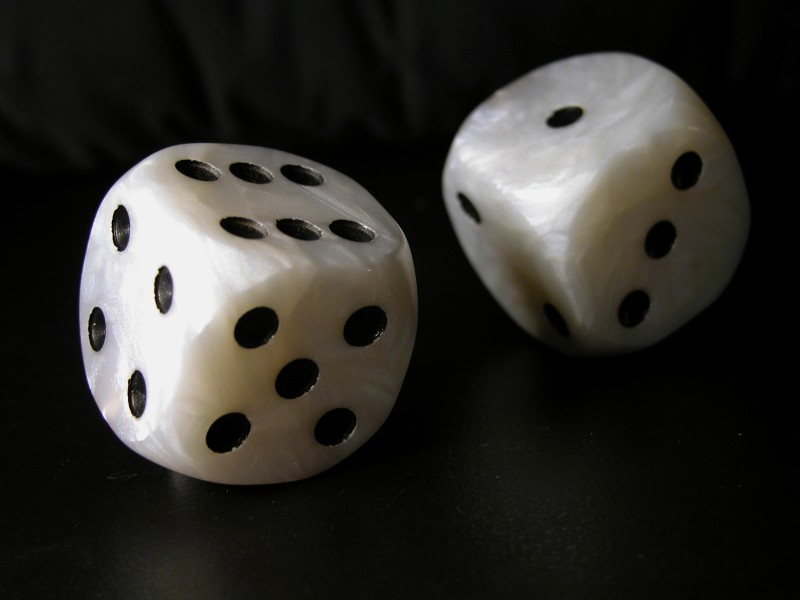
\includegraphics[width=0.5\textwidth]{figures/dice.jpg}
    \caption{Klassische Spielwürfel (aus \cite{wiki:wuerfel}, wie man
    solche Quellenangaben macht lernt ihr später!)}
    \label{fig:wuerfel}
\end{figure}
\begin{Verbatim}[frame=single]
\begin{figure}[h]
    \centering
    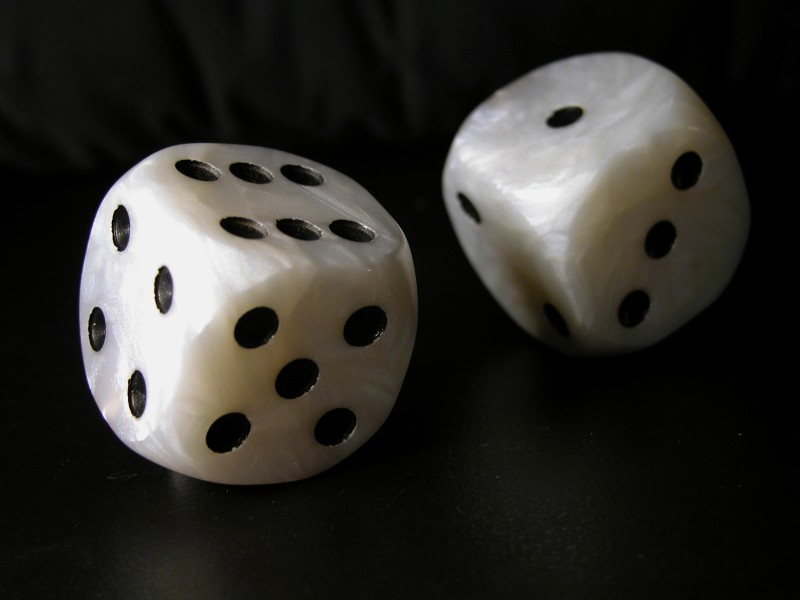
\includegraphics[width=0.5\textwidth]{figures/dice.jpg}
    \caption{Klassische Spielwürfel (aus \cite{wiki:wuerfel}, wie man
    solche Quellenangaben macht lernt ihr später!)}
    \label{fig:wuerfel}
\end{figure}
\end{Verbatim}
Nicht vergessen, mit \verb!\ref{fig:wuerfel}! auf die Abbildung 
\ref{fig:wuerfel} zu verweisen!\\
\lipsum[8-10]
Mehrere Bilder in einer Float sehen auch oft gut aus, wie in Abbildung
\ref{fig:wuerfels} zu sehen. Dort gibt es \ref{fig:wuerfel1} und
\ref{fig:wuerfel2}.\\
\begin{figure}[h]
    \begin{subfigure}[h]{0.49\textwidth}
        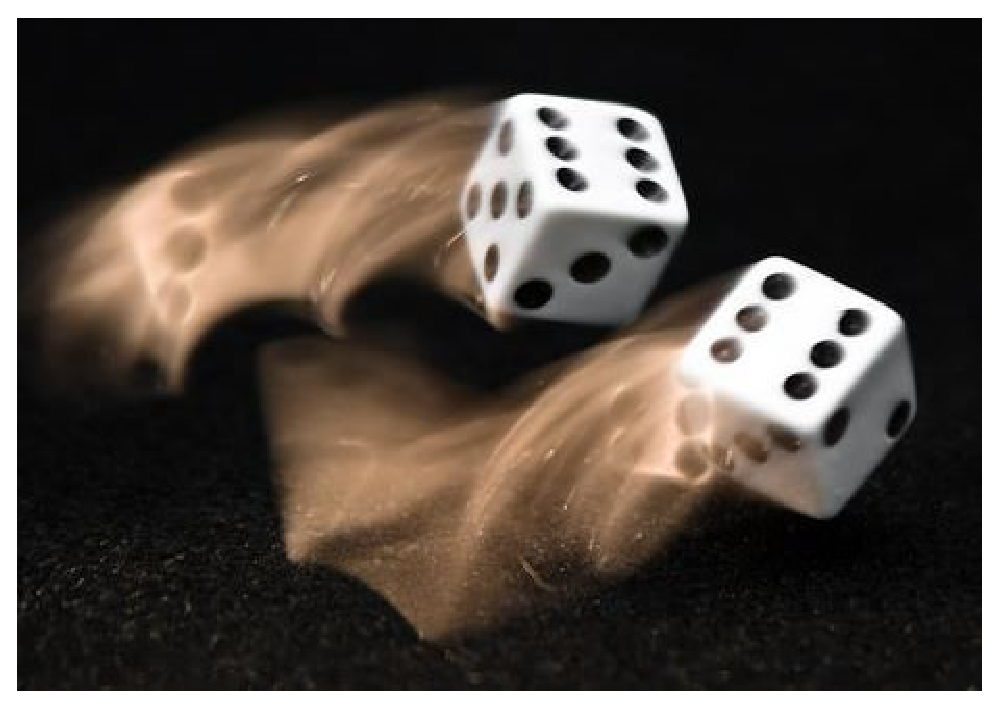
\includegraphics[width=\textwidth]{figures/bildwuerfel1}
        \caption{Erstes Würfelbild}
        \label{fig:wuerfel1}
    \end{subfigure}
    \hfill
    \begin{subfigure}[h]{0.49\textwidth}
        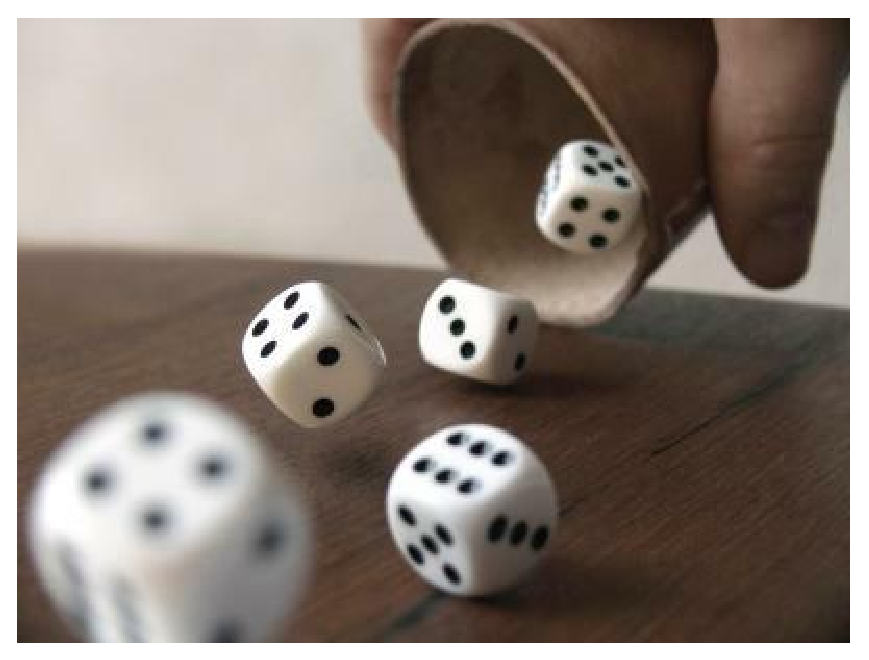
\includegraphics[width=\textwidth]{figures/bildwuerfel2}
        \caption{Zweites Würfelbild}
        \label{fig:wuerfel2}
    \end{subfigure}
    \caption{Mehrere Bilder in einer Figure mit dem Subcaption Package.}
    \label{fig:wuerfels}
\end{figure}
\cprotect\fbox{
    \begin{minipage}{\textwidth}
        \begin{Verbatim}
\usepackage{subcaption}

\begin{figure}[h]
    \begin{subfigure}[h]{0.49\textwidth}
        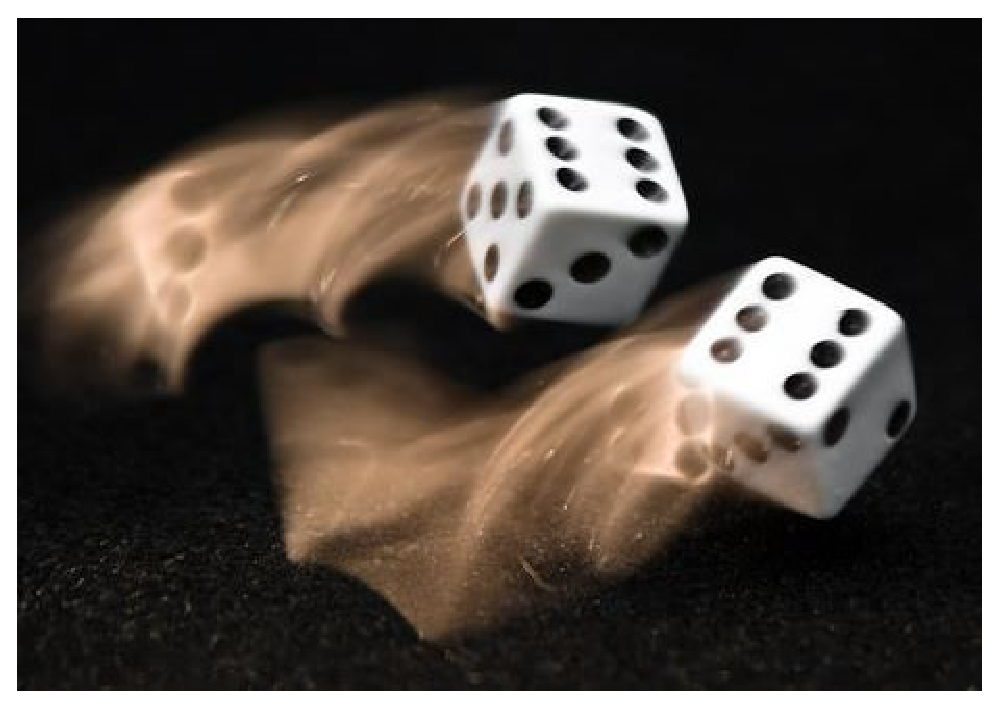
\includegraphics[width=\textwidth]{figures/bildwuerfel1}
        \caption{Erstes Würfelbild}
        \label{fig:wuerfel1}
    \end{subfigure}
    \hfill
    \begin{subfigure}[h]{0.49\textwidth}
        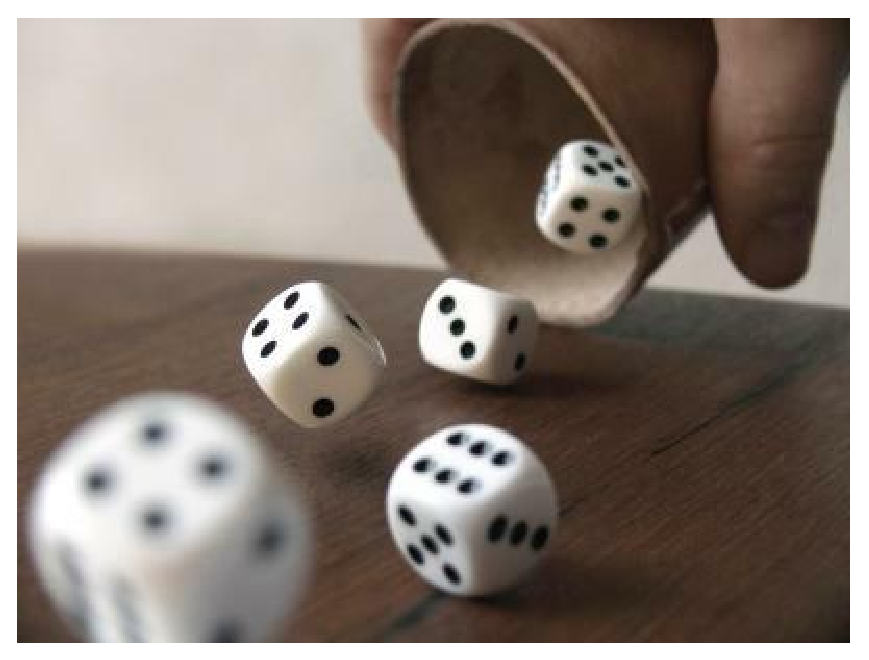
\includegraphics[width=\textwidth]{figures/bildwuerfel2}
        \caption{Zweites Würfelbild}
        \label{fig:wuerfel2}
    \end{subfigure}
    \caption{Gesamtbild-Unterschrift}
    \label{fig:wuerfels}
\end{figure}
        \end{Verbatim}
    \end{minipage}
}

\section{Versuchsaufbau und Ergebnisse}
\cprotect\fbox{
    \begin{minipage}{\textwidth}
        Wichtige Befehle hier:
        \begin{itemize}
            \item \verb!\begin{table}! (float Umgebung)
            \item \verb!\begin{tabular}! (die eigentliche Tabelle)
            \item \verb!\caption{text}! (Tabellenunterschrift)
        \end{itemize}
    \end{minipage}
}\\ \\
Unser Versuchsaufbau ist sehr simpel: Wir werfen einen sechsseitigen
Würfel 600 Mal und tragen die Ergebnisse in einer \textit{Tabelle} ein, nämlich in
Tabelle~\ref{tab:wuerfelwurf}.
\begin{table}[h]
    \centering
    \begin{tabular}{c|l|l}
        Zahl & Anzahl & Anteil\\
        \hline
        1 & 100 & 1/6\\
        2 & 102 & 0,17\\ 
        3 & 99 & 0,165\\
        4 & 100 & 1/6\\
        5 & 98 & 0,16$\overline{3}$\\
        6 & 101 & 0,168$\overline{3}$
    \end{tabular}
    \caption{Ergebnisse von 600 Würfen}
    \label{tab:wuerfelwurf}
\end{table}
\begin{Verbatim}[frame=single]
\begin{table}[h]
    \centering
    \begin{tabular}{c|l|l}    % | vertikale Linie
                              % c center, l linksbündig, r rechtsbündig
        Zahl & Anzahl & Anteil\\
        \hline                % horizontale Linie
        1 & 100 & 1/6\\
        2 & 102 & 0,17\\ 
        3 & 99  & 0,165\\
        4 & 100 & 1/6\\
        5 & 98  & 0,16$\overline{3}$\\
        6 & 101 & 0,168$\overline{3}$ 
    \end{tabular}
    \caption{Ergebnisse von 600 Würfen}
    \label{tab:wuerfelwurf}
\end{table}
\end{Verbatim}
Auf die Tabelle~\ref{tab:wuerfelwurf} verweisen geht dann mit 
\verb!Tabelle~\ref{tab:wuerfelwurf}!. Die Tilde~\verb!~! ist ein Leerzeichen, 
das nicht umgebrochen werden kann, weil das sonst eventuell nicht gut aussieht.
\begin{center}
\fbox{
\begin{minipage}{0.3\textwidth}
    Banan wie man in Tabelle \ref{tab:wuerfelwurf} sehen kann\dots
\end{minipage}
}
\fbox{
\begin{minipage}{0.3\textwidth}
    Banan wie man in Tabelle~\ref{tab:wuerfelwurf} sehen kann\dots
\end{minipage}
}
\end{center}

\section{Einschub: Meine erste Gleichung in \LaTeX{}}
\begin{equation}
    E = m c^2
\end{equation}
\cprotect\fbox{
    \begin{minipage}{1.1\textwidth}
\LaTeX{}-Code dafür:
\begin{Verbatim}
 \begin{equation}
    E = m c^2
 \end{equation}
\end{Verbatim}
    \end{minipage}
}\\ \\ 
\begin{equation}
    \vec{x} = \sum\limits_{i = 1}^{n} x_i \vec{e}_i
\end{equation}
\cprotect\fbox{
    \begin{minipage}{1.1\textwidth}
\LaTeX{}-Code dafür:
\begin{Verbatim}
 \begin{equation}
    \vec{x} = \sum\limits_{i = 1}^{n} x_i \vec{e}_i
 \end{equation}
\end{Verbatim}
    \end{minipage}
}\\ \\ 


\section{Wahrscheinlichkeitsverteilungen}
Eigentlich sollte dieser Abschnitt in den Theorieteil, aber um \LaTeX{} zu
lernen ist es wohl sinnvoller, erst Text und dann mathematische Ausdrücke
zu lernen.

Wenn wir den Würfelwurf so interpretieren, dass man bei einer "`6"' gewinnt
und ansonsten verliert (Erfolg oder Misserfolg), dann haben wir einen
sogenannten \textit{Bernoulli-Prozess}, welcher durch die
\textit{Binomialverteilung} \cite{wiki:binomial} beschrieben wird. 
\begin{figure}
    \centering
    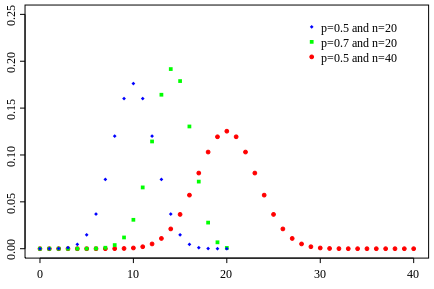
\includegraphics[width=0.8\textwidth]{figures/binomial.png}
    \caption{Die Binomialverteilung für verschiedene Werte von $p$
    (aus \cite{wiki:binomial})}
    \label{fig:binomialverteilung}
\end{figure}
Ein Plot der Binomialvertilung für verschiedene Wahrscheinlichkeiten
$p$ ist in Abbildung~\ref{fig:binomialverteilung} gegeben.
\begin{quote}
    Ist $p$ die Erfolgswahrscheinlichkeit bei einem Versuch und $n$ die Anzahl der
    Versuche, dann bezeichnet man mit $B(k \mid p,n)$, $B_{n,p}(k)$, $B(n,p,k)$
    oder $B(n;p;k)$ die Wahrscheinlichkeit, genau $k$ Erfolge zu erzielen 
    (aus \cite{wiki:binomial}).
\end{quote}
Die Wahrscheinlichkeit für genau $k$ Treffer ist gegeben durch
\begin{equation}
    B(k | p,n) = \binom {n}{k} p^k (1-p)^{n-k}\quad \text{für}\quad k=0,1,\dots, n,
    \label{eq:binomial}
\end{equation}
für $n$ Versuche mit der Trefferwahrscheinlichkeit $p\in [0,1]$.\\
\\
\cprotect\fbox{
    \begin{minipage}{1.1\textwidth}
\LaTeX{}-Code dafür:
\begin{Verbatim}
 \begin{equation}
   B(k|p,n) = \binom {n}{k} p^k (1-p)^{n-k}\quad \text{für}\quad k=0,1,\dots, n,
   \label{eq:binomial}
 \end{equation}
\end{Verbatim}
    \end{minipage}
}\\ \\ 
Natürlich kann man dann auf die Gleichung (\ref{eq:binomial}) mit 
\verb!Gleichung~(\ref{eq:binomial})! verweisen und \verb!\pageref{eq:binomial}! sagt
uns, dass die Gleichung auf Seite \pageref{eq:binomial} ist.

Der Erwartungswert $\mu$ errechnet sich durch $\mu=\sum_{i=1}^n x_i p_i$, also
\begin{align}
    \mu &= \sum_{k=0}^n k \binom nk p^k (1-p)^{n-k}\\
        &= \dots \nonumber\\
        &= np\quad.
    \label{eq:erwartungswert}
\end{align}
Bei einer (kontinuierlichen) Wahrscheinlichkeitsverteilung muss man zu
Integralen übergehen:
Um die Wahrscheinlichkeit, dass ein Wert $x$ im Bereich $\mu \pm j\sigma$
liegt, zu bekommen, integriert man über die Verteilungsfunktion $P(x,\mu)$
\begin{equation}
    W(\mu, \sigma) = \int_{\mu-j\sigma}^{\mu+j\sigma} P(x,\mu) \mathrm{d}x\quad.
    \label{eq:Standardabweichung}
\end{equation}
Ist $P(x,\mu)$ die Normalverteilung, so erhält man 
\begin{tabular}{lcrl}
					$\mu$ & $\pm$&$\sigma$: & $W=0.683$  \\ 
					$\mu $&$\pm$&$2\sigma$: & $W=0.955$  \\ 
					$\mu $&$\pm$&$3\sigma$: & $W=0.997$ 
\end{tabular},\\
das sind die sogenannten Standardabweichungen.\\
\\
\begin{Verbatim}[frame=single]
Ist $P(x,\mu)$ die Normalverteilung, so erhält man 
\begin{tabular}{lcrl}
    $\mu$ & $\pm$ & $ \sigma$: & $W=0.683$  \\ 
    $\mu$ & $\pm$ & $2\sigma$: & $W=0.955$  \\ 
    $\mu$ & $\pm$ & $3\sigma$: & $W=0.997$ 
\end{tabular},\\

% \pm steht für plusminus
\end{Verbatim}
~\\
\cprotect\fbox{
    \begin{minipage}{\textwidth}
Wichtige Befehle in diesem Abschnitt:
\begin{Verbatim}
\begin{quote} . . . \end{quote}
\begin{equation} . . . \end{equation}
\begin{align} . . . \end{align}
\sum_{k=0}^n \int_{0}^{\infty} \quad \dots \dotsc \cdots
\mu \sigma \mathrm{d}x \pm
\end{Verbatim}
    \end{minipage}
}
\cprotect\fbox{
    \begin{minipage}{1.1\textwidth}
        Weitere wichtige Mathe-Befehle:\\
        Inline Mathe Formeln mit \verb!$\mu$!\\\\
        $\left( \frac{\frac{1}{2} + 1}{3} \right) \neq ( \frac{\frac{1}{2} + 1}{3} )$\\
        \verb!$\left(\frac{\frac{1}{2}+1}{3}\right) \neq (\frac{\frac{1}{2}+1}{3})!\\
        \\
        $\pi \in \mathbb R$ \\
        \verb!\pi \in \mathbb R! \\
        \\
        $\mathbf{F}_C = \frac{1}{4 \pi \epsilon_0}\frac{q_1 q_2}{r^3}\mathbf{\hat{r}}$\\
        \verb!\mathbf{F}_C = \frac{1}{4 \pi \epsilon_0}\frac{q_1 q_2}{r^3}\mathbf{\hat{r}}!
        \\ \\
        $\vec{v}$\\
        \verb!\vec{v}!\\\\
        $\underbrace{1 + 2}_3$\\
        \verb!\underbrace{1 + 2}_3!\\\\

        Mit dem bm Package: kursive fette Buchstaben $a B ~ \mathbf{a} \mathbf{B} ~ \bm{a} \bm{B}$
    \end{minipage}
}
        
\section{Versuchsauswertung}
\lipsum[1]
\begin{equation}
    \begin{pmatrix}
        a_1 & a_2 & a_3 & a_4 \\
        b_1 & b_2 & b_3 & b_4 \\
        c_1 & c_2 & c_3 & c_4 \\
        d_1 & d_2 & d_3 & d_4
    \end{pmatrix}
    \quad \text{und} \quad
    \begin{bmatrix}
        1       & 0     & \dots  & 0      \\
        0       & 1     & \dots  & 0      \\
        \vdots  & 0     & \ddots & \vdots \\
        0       & \dots & 0      & 1
    \end{bmatrix}
\end{equation}
\begin{Verbatim}[frame=single]
\begin{equation}
    \begin{pmatrix}
        a_1 & a_2 & a_3 & a_4 \\
        b_1 & b_2 & b_3 & b_4 \\
        c_1 & c_2 & c_3 & c_4 \\
        d_1 & d_2 & d_3 & d_4
    \end{pmatrix}
    \quad \text{und} \quad
    \begin{bmatrix}
        1       & 0     & \dots  & 0      \\
        0       & 1     & \dots  & 0      \\
        \vdots  & 0     & \ddots & \vdots \\
        0       & \dots & 0      & 1
    \end{bmatrix}
\end{equation}
\end{Verbatim}

\begin{itemize}
    \item matrix (nackte Matrix)
    \item bmatrix \{\}
    \item Bmatrix []
    \item pmatrix ()
    \item vmatrix || ||
    \item Vmatrix | |
    \item Bordermatrix
\end{itemize}
\section{Zusammenfassung und Ausblick}
Wir haben also gesehen, dass
\begin{itemize}
    \item \LaTeX{} cool ist,
    \item man damit einfach größere Dokumente strukturieren kann,
        weil \LaTeX{} sich um das meiste kümmert
    \item und dass man mathematische Formeln so relativ einfach setzen kann.
        Die \LaTeX{} Syntax dafür ist im Internet\footnote{zum Beispiel
        auf \url{https://www.reddit.com/r/Physics/}} sehr weit verbreitet und
        wird auch außerhalb von .tex Dokumenten häufig verwendet.
\end{itemize}
\lipsum[2]




%%%%%%%%%%%%%%%%%%%%%%%%%%%%%%%%%%%%%%%%%%%%%%%%%%%%%%%%%%%%%%%%%%%%%%%%%%%
%Abbildungsverzeichnis
%%%%%%%%%%%%%%%%%%%%%%%%%%%%%%%%%%%%%%%%%%%%%%%%%%%%%%%%%%%%%%%%%%%%%%%%%%%
\addcontentsline{toc}{section}{Abbildungsverzeichnis}
\newpage
\listoffigures 
~\\
\cprotect\fbox{
    \begin{minipage}{\textwidth}
\begin{verbatim}
\newpage
\addcontentsline{toc}{section}{Abbildungsverzeichnis}
\listoffigures 
\newpage
\end{verbatim}
addcontentsline fügt ins Inhaltsverzeichnis\footnote{toc, table of contents}
etwas ein.\\
    \end{minipage}
}
%\newpage
%%%%%%%%%%%%%%%%%%%%%%%%%%%%%%%%%%%%%%%%%%%%%%%%%%%%%%%%%%%%%%%%%%%%%%%%%%%
%Literaturverzeichnis
%%%%%%%%%%%%%%%%%%%%%%%%%%%%%%%%%%%%%%%%%%%%%%%%%%%%%%%%%%%%%%%%%%%%%%%%%%%
\addcontentsline{toc}{section}{Literaturverzeichnis} 
\begin{thebibliography}{abc}
    \bibitem{wiki:wuerfel} Wikipedia (2016) Spielwürfel (www-site)
        \url{https://de.wikipedia.org/wiki/Spielwürfel}
    \bibitem{wiki:binomial} Wikipedia (2016) Binomialverteilung (www-site)
        \url{https://de.wikipedia.org/wiki/Binomialverteilung}
\end{thebibliography}
\cprotect\fbox{
    \begin{minipage}{\textwidth}
\begin{Verbatim}
\addcontentsline{toc}{section}{Literaturverzeichnis} 
\begin{thebibliography}{abc}
    \bibitem{wiki:wuerfel} Wikipedia(2016) Spielwürfel (www-site)
        \url{https://de.wikipedia.org/wiki/Spielwürfel}
    \bibitem{wiki:binomial} Wikipedia (2016) Binomialverteilung (www-site)
        \url{https://de.wikipedia.org/wiki/Binomialverteilung}
\end{thebibliography}
\end{Verbatim}
~\\
Im Text kann man dann mit \verb!\cite{wiki:wuerfel}! verweisen.\\
Für \verb!\url{}! ist \verb!\usepackage{hyperref}! nötig!
    \end{minipage}
}
\end{document}
